\documentclass[12pt]{report}
\usepackage[top=1in, bottom=1in, left=0.5in, right=0.5in]{geometry}
\usepackage{amsmath, amsfonts, amssymb, libris, enumerate, fancyhdr, xcolor, lipsum, titling, minted, algorithm, algpseudocode, algorithmicx, float, hyperref, booktabs, graphicx, array}
\usepackage[utf8]{inputenc}

\usepackage[Glenn]{fncychap}
\usepackage[skip=20pt, indent=30pt]{parskip}
\usepackage{setspace}
\onehalfspacing

\usepackage[some]{background}

\definecolor{titlepagecolor}{cmyk}{.02,.04,0,.90}

\DeclareFixedFont{\bigsf}{T1}{phv}{b}{n}{1.5cm}
% Default fixed font does not support bold face
\DeclareFixedFont{\ttb}{T1}{txtt}{bx}{n}{12} % for bold
\DeclareFixedFont{\ttm}{T1}{txtt}{m}{n}{12}  % for normal

% Custom colors
\usepackage{color}
\definecolor{deepblue}{rgb}{0,0,0.5}
\definecolor{deepred}{rgb}{0.6,0,0}
\definecolor{deepgreen}{rgb}{0,0.5,0}

\usepackage{listings}

% Python style for highlighting
\newcommand\pythonstyle{\lstset{
language=Python,
basicstyle=\ttm,
morekeywords={self},              % Add keywords here
keywordstyle=\ttb\color{deepblue},
emph={MyClass,__init__},          % Custom highlighting
emphstyle=\ttb\color{deepred},    % Custom highlighting style
stringstyle=\color{deepgreen},
frame=tb,                         % Any extra options here
showstringspaces=false,
tabsize=2,
}}


% Python environment
\lstnewenvironment{python}[1][]
{
\pythonstyle
\lstset{#1}
}
{}

% Python for external files
\newcommand\pythonexternal[2][]{{
\pythonstyle
\lstinputlisting[#1]{#2}}}

% Python for inline
\newcommand\pythoninline[1]{{\pythonstyle\lstinline!#1!}}


\makeatletter
\renewcommand{\@chapapp}{Section}
\makeatother
\renewcommand{\thechapter}{\Roman{chapter}}

\pagestyle{fancy}
% \fancyhead[l]{Final Project Report \\}
\fancyhead[l]{ }
% \fancyhead[r]{Sayan Das: \texttt{B2430035} \\ Raihan Uddin: \texttt{B2430070}}
\fancyfoot[c]{\thepage}
\renewcommand{\headrulewidth}{0.2pt}
\setlength{\headheight}{28pt}

\title{Project 1 Report}
\author{
  Sayan Das
  \and
  Raihan Uddin
}

\begin{document}

\begin{titlepage}
	\newcommand{\HRule}{\rule{\linewidth}{0.5mm}}
	\center


	\textsc{\LARGE \textbf{Ramakrishna Mission Vivekananda Educational and Research Institute}}\\[1.5cm]

	\textsc{\LARGE Computer Vision}\\[0.5cm]

	\textsc{\large Project Report}\\[0.5cm]

	\HRule\\[0.4cm]

	{\huge\bfseries Image Filtering and Hybrid Images}\\[0.4cm]

	\HRule\\[1.5cm]



\large
\textit{Submitted By}\\
\textsc{\textbf{Sayan Das }}\\
\vspace{-0.5em}
\textsc{\texttt{B2430035 }}\\
\textsc{\textbf{Raihan Uddin }}\\
\vspace{-0.5em}
\textsc{\texttt{B2430070} }\\

	~
	\begin{minipage}{0.4\textwidth}
		% \begin{flushright}
		% 	\large
		% 	\textit{Submitted To}\\
		% 	\textbf{\textsc{Br. Bhaswarachaitanya (Tamal Maharaj)}}
		% \end{flushright}
	\end{minipage}


	\vfill\vfill\vfill

	{\large February 10, 2025}

	\vfill

\end{titlepage}
\restoregeometry

\tableofcontents

\chapter{Introduction}
Hybrid images, as introduced by Oliva, Torralba, and Schyns in their SIGGRAPH 2006 paper \cite{oliva2006}, are static images that change interpretation based on viewing distance. This phenomenon leverages the human visual system's multi-scale processing, where high-frequency details dominate perception at close range, while low-frequency components become prominent from afar. The goal of this project is to implement image filtering and hybrid image generation, aligning with the methodology described in the paper.
\section{Motivation}
The primary challenge in creating compelling hybrid images lies in the precise separation and recombination of these frequency components. This requires:
\vspace{-1.25em}
\begin{enumerate}
	\setlength\itemsep{-1.05em}

	\item{\textbf{Accurate Filtering: }}Implementing an image filtering algorithm that can effectively extract low and high-frequency components without introducing artifacts.
	\item{\textbf{Perceptual Alignment: }}Ensuring that the two images are aligned in a way that their frequency components blend seamlessly, avoiding perceptual conflicts.
	\item{\textbf{Parameter Tuning: }}Selecting appropriate cutoff frequencies for the filters to achieve the desired perceptual effect.

\end{enumerate}

\noindent This project aims to address these challenges by implementing a custom image filtering function and using it to generate hybrid images. The goal is to replicate the results described in the paper \cite{oliva2006} and explore the perceptual effects of hybrid images. By doing so, we aim to gain a deeper understanding of multi-scale image processing and its applications in computer vision.

\noindent The problem can be summarized as follows:

\vspace{-1.25em}
\begin{enumerate}
	\setlength\itemsep{-1.05em}

	\item{\textbf{Input: }}Two aligned images - \texttt{Image 1} and \texttt{Image 2} (e.g., \texttt{dog.bmp} and \texttt{cat.bmp}).
	\item{\textbf{Output: }}A hybrid image that changes interpretation based on viewing distance, along with intermediate results (low-frequency and high-frequency components).

\end{enumerate}


\chapter{Methodology}
\section{Image Filtering}
The core of hybrid image creation lies in filtering operations. The custom function \texttt{my\_imfilter} implements 2D convolution with the following steps:

\begin{enumerate}
	\setlength\itemsep{-1.05em}

	\item{\textbf{Padding: }}he input image is padded using zero-padding to preserve spatial dimensions post-convolution. The padding size is determined by the filter dimensions $ (k, l) $ with \label{sec:impadding}
	\begin{equation}
			\begin{aligned}
					pad_k &= \left\lfloor \frac{k}{2} \right\rfloor \\
					pad_l &= \left\lfloor \frac{l}{2} \right\rfloor
			\end{aligned}
	\end{equation}
	\item{\textbf{Convolution: }}For each color channel (RGB), a sliding window extracts image patches, which are element-wise multiplied with the filter and summed to compute the output pixel. Mathematically, \label{sec:imconvolution}
	\[
	O(x, y, c) = \sum_{i=0}^{m-1} \sum_{j=0}^{n-1} \sum_{d=0}^{D-1} I(x + i, y + j, d) \cdot K(i, j, d, c)
	\]

	where:
	\begin{itemize}
		\setlength\itemsep{-1.05em}
			\item \( O(x, y, c) \) is the output pixel value at position \( (x, y) \) for channel \( c \).
			\item \( I(x + i, y + j, d) \) is the input image pixel value at position \( (x + i, y + j) \) for channel \( d \).
			\item \( K(i, j, d, c) \) is the convolution kernel (filter) value at position \( (i, j) \), mapping from input channel \( d \) to output channel \( c \).
			\item \( m \times n \) is the size of the filter (height and width).
			\item \( D \) is the number of input channels (for RGB, \( D = 3 \)).
	\end{itemize}

\end{enumerate}


\section{Hybrid Image Generation}
The function \texttt{create\_hybrid\_image} combines two images:

\vspace{-1.25em}
\begin{enumerate}
	\setlength\itemsep{-1.05em}

	\item{\textbf{Low-Frequency Component: }}Obtained by applying a Gaussian low-pass filter to \texttt{Image 1}.
	$$ I_1 \cdot G_1 $$
	\item{\textbf{High-Frequency Component: }}Derived by subtracting the low-pass filtered version of \texttt{Image 2} from itself.
	$$ I_2 \cdot (1 - G_2) $$
	\item{\textbf{Hybrid Image: }}The sum of low and high frequencies, clipped to [0, 1] to maintain valid pixel intensities.
	$$ H = I_1 \cdot G_1 + I_2 \cdot (1 - G_2) $$

\end{enumerate}

\chapter{Implementation}
\section{Tools and Libraries}
The tools and libraries used for this project are:
\vspace{-1.25em}
\begin{enumerate}
    \setlength\itemsep{-1.05em}
    \item{\textbf{Python:}} The primary programming language for this project.
    \item{\textbf{Jupyter Notebook:}} For interactive code development.
    \item{\textbf{Libraries:}}
        \vspace{-1.5em}
        \begin{enumerate}
            \setlength\itemsep{-1.5em}
            \item{\textbf{Numpy:}} For numerical operations like array sums, and for faster mathematical computations.
						\item{\textbf{Matplotlib:}} For displaying images and visualizing filters.
						\item{\textbf{CV2:}} For image processing tasks such as reading, writing, and manipulating images.
				\end{enumerate}
\end{enumerate}

\section{Implementation Details}
\subsection{\texttt{ my\_imfilter } function}
Before constructing a hybrid image, we need a function to apply a filter to an image. The function \texttt{my\_imfilter(image, filter)} does this by:
\begin{enumerate}
	\setlength\itemsep{-1.05em}

	\item{\textbf{Padding the Image: }} Since filtering requires accessing pixels around each center pixel, we pad the input image using \pythoninline{np.pad}. The padding size is determined following the process mentioned in methodology \ref{sec:impadding}. \\ \textit{Unlike how it was mentioned in the documentation, we used k × l filter, to support rectangular kernels.}
	\item{\textbf{Applying the Filter: }} For each pixel in the image, a window of size $ (k \times l) $ is extracted.This window is element-wise multiplied with the filter and summed to get the new pixel value. This operation is repeated across all three color channels (R, G, B). \ref{sec:imconvolution}. We used \pythoninline{np.sum} for faster computation.

\end{enumerate}
The function returns the filtered image, where each pixel is computed using the convolution operation.

\subsection{\texttt{ create\_hybrid\_image } function}
The \textbf{hybrid image} is constructed by combining the low-frequency content of one image and the high-frequency content of another.

\begin{enumerate}
	\setlength\itemsep{-1.05em}
\item{Step 1: Extract Low-Frequency Content}
We obtain the \textbf{low-frequency} content of \texttt{image1} by filtering it with a low-pass filter:
\[
\text{low\_frequencies} = \text{my\_imfilter}(\text{image1}, \text{filter})
\]
A low-pass filter (e.g., a Gaussian blur) removes high-frequency details, leaving only smooth variations.
\item{Step 2: Extract High-Frequency Content}
The high-frequency content of \texttt{image2} is obtained by subtracting its low-frequency component:
\[
\text{high\_frequencies} = \text{image2} - \text{my\_imfilter}(\text{image2}, \text{filter})
\]
This step removes smooth regions and enhances sharp edges and fine details.
\item{Step 3: Combine Both Components}
Finally, the \textbf{hybrid image} is formed by adding the low-frequency and high-frequency components:
\[
\text{hybrid\_image} = \text{low\_frequencies} + \text{high\_frequencies}
\]
Since pixel values must be between \( 0 \) and \( 1 \) (for correct image representation), we apply \textbf{clipping}:
\[
\text{hybrid\_image} = \text{np.clip}(\text{hybrid\_image}, 0, 1)
\]
\end{enumerate}

The hybrid image contains \textbf{smooth variations} from \texttt{image1} and \textbf{sharp details} from \texttt{image2}. When viewed \textbf{up close}, the high-frequency details dominate (showing \texttt{image2}). When viewed \textbf{from a distance}, the low-frequency content dominates (showing \texttt{image1}).

\subsection{Creating the filter}
We used \pythoninline{cv2.getGaussianKernel(ksize, sigma)} to generate a 1D Gaussian kernel (column vector). We muliplied it with its transpose (filter @ filter.T) to convert it into a 2D Gaussian kernel. This method leverages separability, making Gaussian blurring more efficient than computing a full 2D kernel directly.

\chapter{Results}
\section{Cat-Dog Hybrid Image}
\vspace{1.25em}
\begin{figure}[H]
	\centering
	\begin{minipage}{0.45\textwidth}
			\centering
			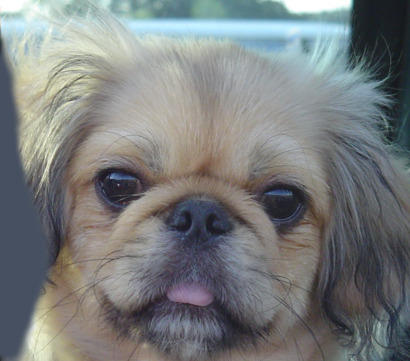
\includegraphics[height=12em]{./images/dog.jpg}
		\end{minipage}
		\begin{minipage}{0.45\textwidth}
			\centering
			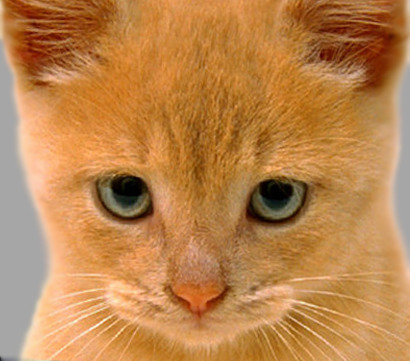
\includegraphics[height=12em]{./images/cat.jpg}
		\end{minipage}
		\caption{Original Dog and Cat Image}
		\label{dog_cat}
\end{figure}
\begin{figure}[H]
	\centering
	\begin{minipage}{0.45\textwidth}
			\centering
			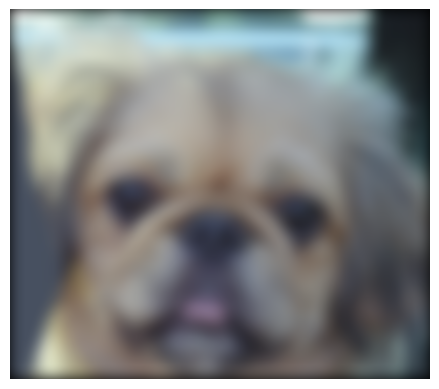
\includegraphics[height=12em]{./images/dog_low.png}
		\end{minipage}
		\begin{minipage}{0.45\textwidth}
			\centering
			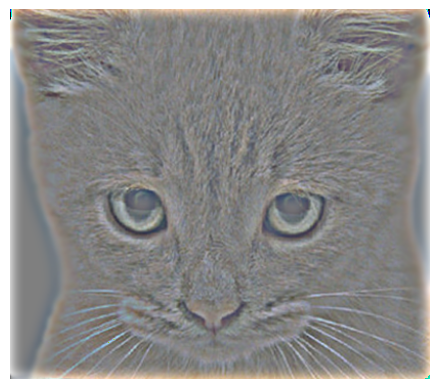
\includegraphics[height=12em]{./images/cat_high.png}
		\end{minipage}
		\caption{Low Frequency Dog and High Frequency Cat Image generated with cutoff-frequency=7}
		\label{dog_cat_low_high}
\end{figure}
\begin{figure}[H]
	\centering
		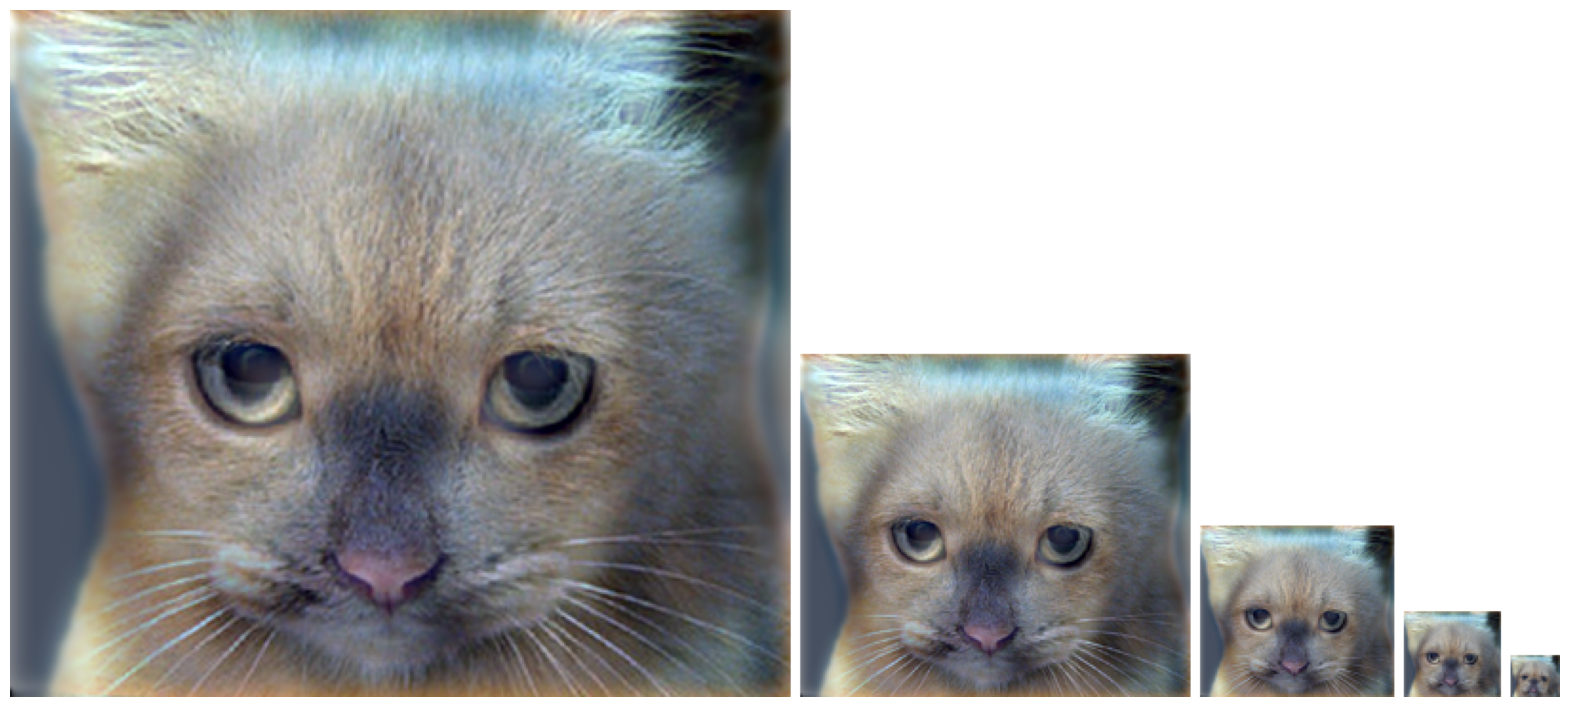
\includegraphics[height=15em]{./images/dog_cat_hybrid.png}
		\caption{Dog cat Hybrid Image}
		\label{dog_cat_low_hybrid}
\end{figure}
\section{Bicycle-Motorcycle Hybrid Image}
\vspace{1.25em}
\begin{figure}[H]
    \centering
    \begin{minipage}{0.45\textwidth}
            \centering
            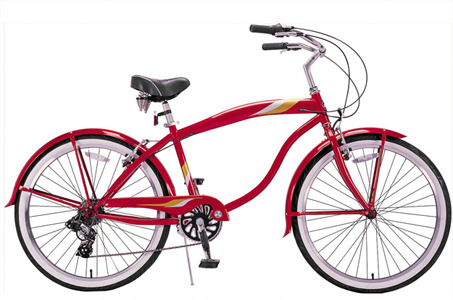
\includegraphics[height=12em]{./images/bicycle.jpg}
        \end{minipage}
        \begin{minipage}{0.45\textwidth}
            \centering
            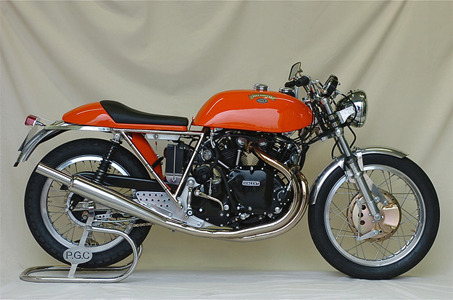
\includegraphics[height=12em]{./images/motorcycle.jpg}
        \end{minipage}
        \caption{Original Bicycle and Motorcycle Image}
        \label{bicycle_motorcycle}
\end{figure}
\begin{figure}[H]
    \centering
    \begin{minipage}{0.45\textwidth}
            \centering
            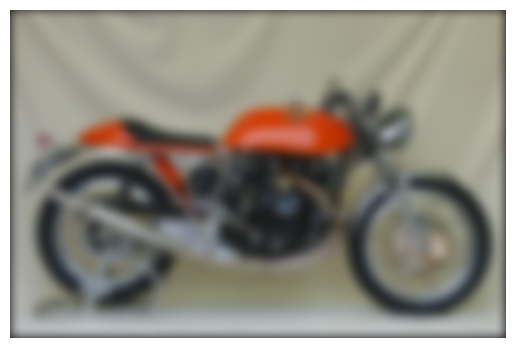
\includegraphics[height=12em]{./images/motorcycle_low.png}
        \end{minipage}
        \begin{minipage}{0.45\textwidth}
            \centering
            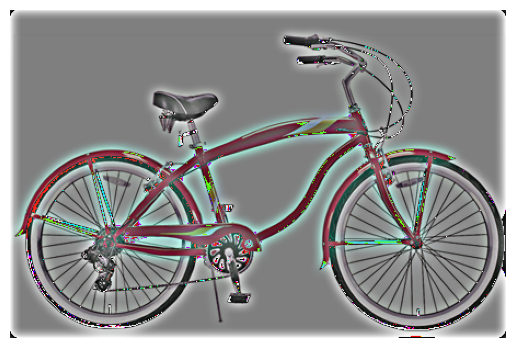
\includegraphics[height=12em]{./images/bicycle_high.png}
        \end{minipage}
        \caption{Low Frequency Bicycle and High Frequency Motorcycle Image generated with cutoff-frequency=5}
        \label{bicycle_motorcycle_low_high}
\end{figure}
\begin{figure}[H]
    \centering
        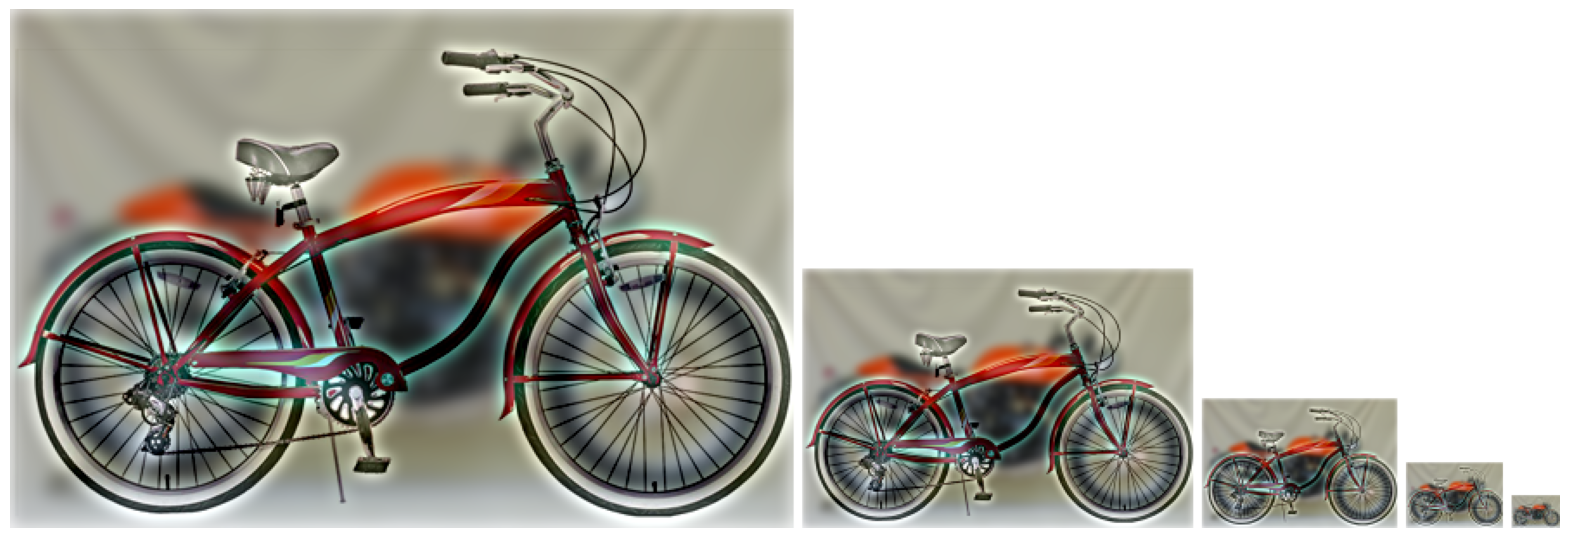
\includegraphics[height=15em]{./images/motorcycle_bicycle_hybrid.png}
        \caption{Bicycle Motorcycle Hybrid Image}
        \label{bicycle_motorcycle_hybrid}
\end{figure}

\section{Plane-Bird Hybrid Image}
\vspace{1.25em}
\begin{figure}[H]
    \centering
    \begin{minipage}{0.45\textwidth}
            \centering
            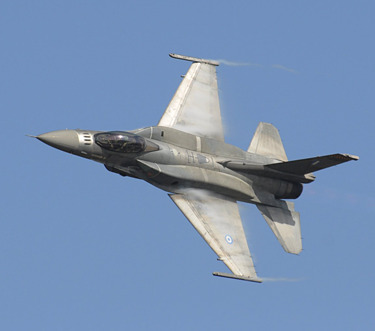
\includegraphics[height=12em]{./images/plane.jpg}
        \end{minipage}
        \begin{minipage}{0.45\textwidth}
            \centering
            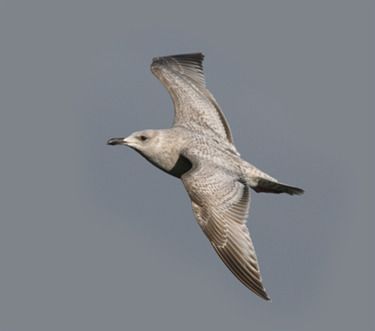
\includegraphics[height=12em]{./images/bird.jpg}
        \end{minipage}
        \caption{Original Plane and Bird Image}
        \label{plane_bird}
\end{figure}
\begin{figure}[H]
    \centering
    \begin{minipage}{0.45\textwidth}
            \centering
            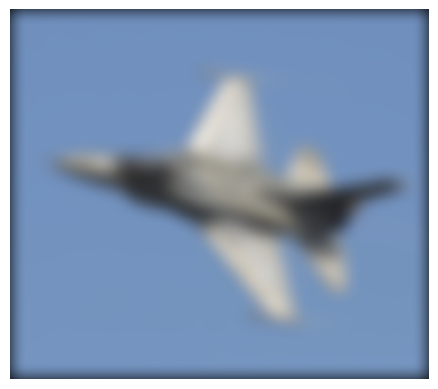
\includegraphics[height=12em]{./images/plane_low.png}
        \end{minipage}
        \begin{minipage}{0.45\textwidth}
            \centering
            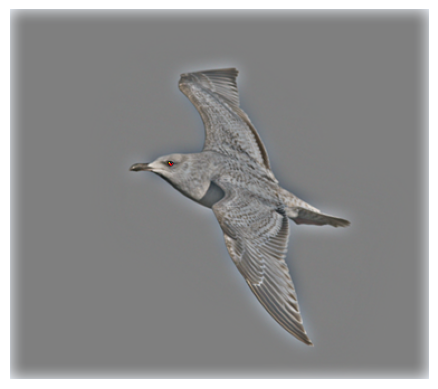
\includegraphics[height=12em]{./images/bird_high.png}
        \end{minipage}
        \caption{Low Frequency Plane and High Frequency Bird Image generated with cutoff-frequency=7}
        \label{plane_bird_low_high}
\end{figure}
\begin{figure}[H]
    \centering
        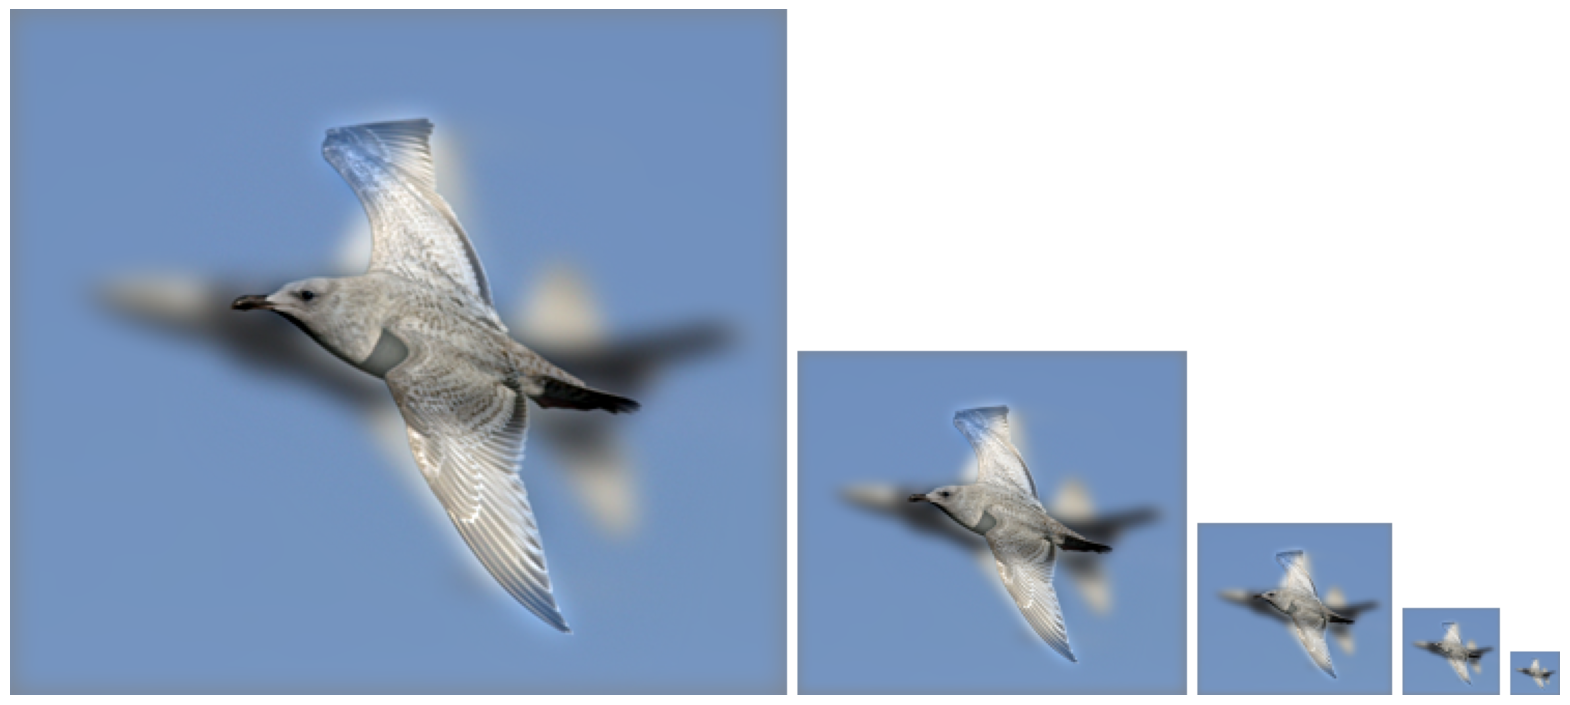
\includegraphics[height=15em]{./images/plane_bird_hybrid.png}
        \caption{Plane Bird Hybrid Image}
        \label{plane_bird_hybrid}
\end{figure}

\section{Einstein-Marilyn Hybrid Image}
\vspace{1.25em}
\begin{figure}[H]
    \centering
    \begin{minipage}{0.45\textwidth}
            \centering
            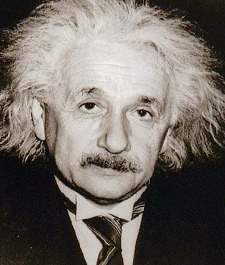
\includegraphics[height=12em]{./images/einstein.jpg}
        \end{minipage}
        \begin{minipage}{0.45\textwidth}
            \centering
            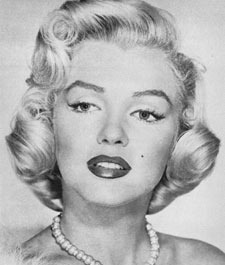
\includegraphics[height=12em]{./images/marilyn.jpg}
        \end{minipage}
        \caption{Original Einstein and Marilyn Image}
        \label{einstein_marilyn}
\end{figure}
\begin{figure}[H]
    \centering
    \begin{minipage}{0.45\textwidth}
            \centering
            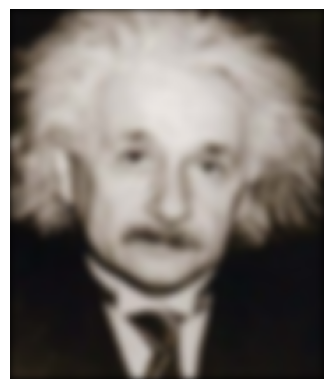
\includegraphics[height=12em]{./images/einstein_low.png}
        \end{minipage}
        \begin{minipage}{0.45\textwidth}
            \centering
            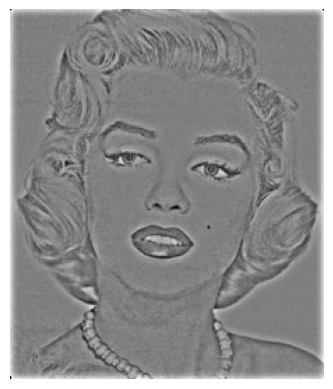
\includegraphics[height=12em]{./images/marilyn_high.png}
        \end{minipage}
        \caption{Low Frequency Einstein and High Frequency Marilyn Image generated with cutoff-frequency=3}
        \label{einstein_marilyn_low_high}
\end{figure}
\begin{figure}[H]
    \centering
        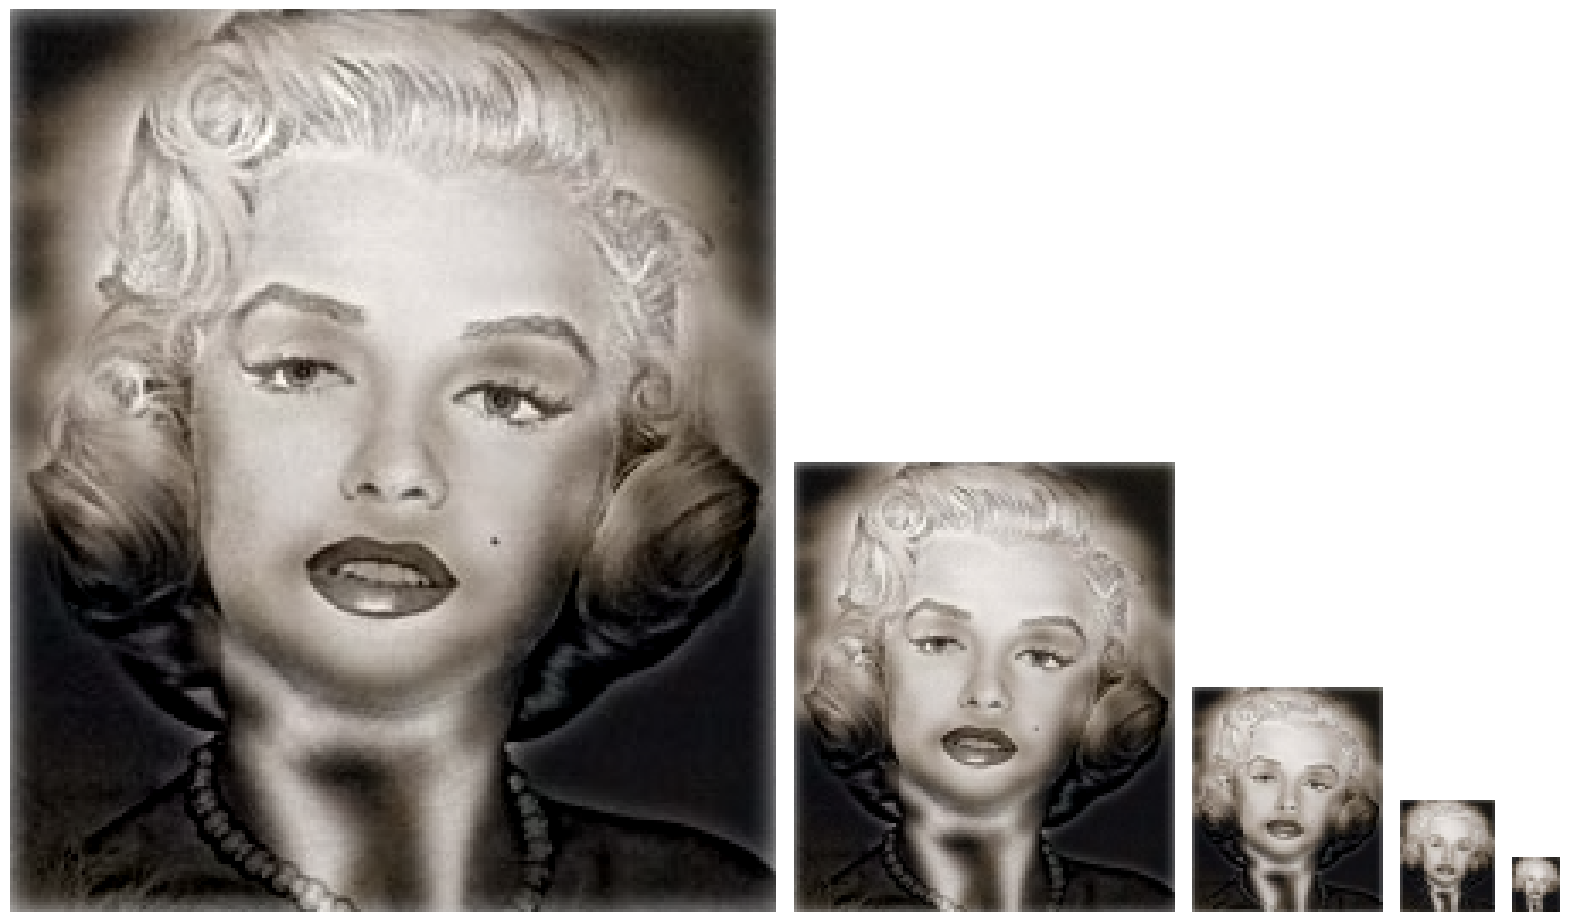
\includegraphics[height=15em]{./images/einstein_marilyn_hybrid.png}
        \caption{Einstein Marilyn Hybrid Image}
        \label{einstein_marilyn_hybrid}
\end{figure}

\section{Submarine-Fish Hybrid Image}
\vspace{1.25em}
\begin{figure}[H]
    \centering
    \begin{minipage}{0.45\textwidth}
            \centering
            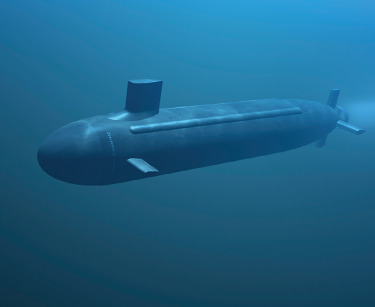
\includegraphics[height=12em]{./images/submarine.jpg}
        \end{minipage}
        \begin{minipage}{0.45\textwidth}
            \centering
            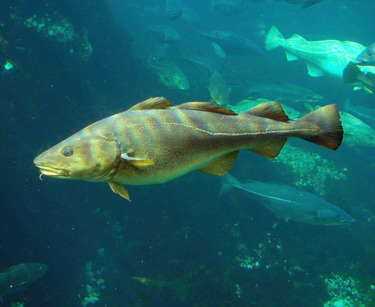
\includegraphics[height=12em]{./images/fish.jpg}
        \end{minipage}
        \caption{Original Submarine and Fish Image}
        \label{submarine_fish}
\end{figure}
\begin{figure}[H]
    \centering
    \begin{minipage}{0.45\textwidth}
            \centering
            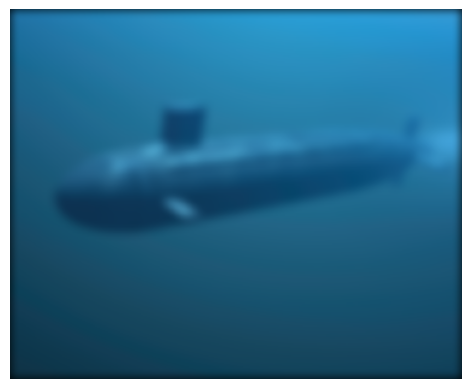
\includegraphics[height=12em]{./images/submarine_low.png}
        \end{minipage}
        \begin{minipage}{0.45\textwidth}
            \centering
            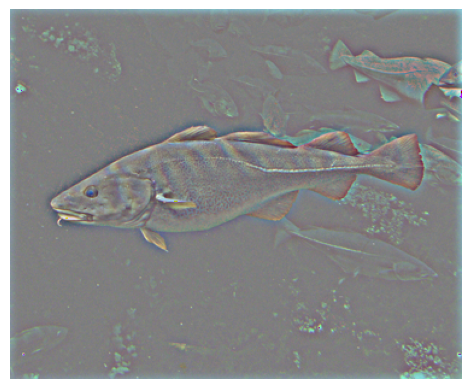
\includegraphics[height=12em]{./images/fish_high.png}
        \end{minipage}
        \caption{Low Frequency Submarine and High Frequency Fish Image generated with cutoff-frequency=4}
        \label{submarine_fish_low_high}
\end{figure}
\begin{figure}[H]
    \centering
        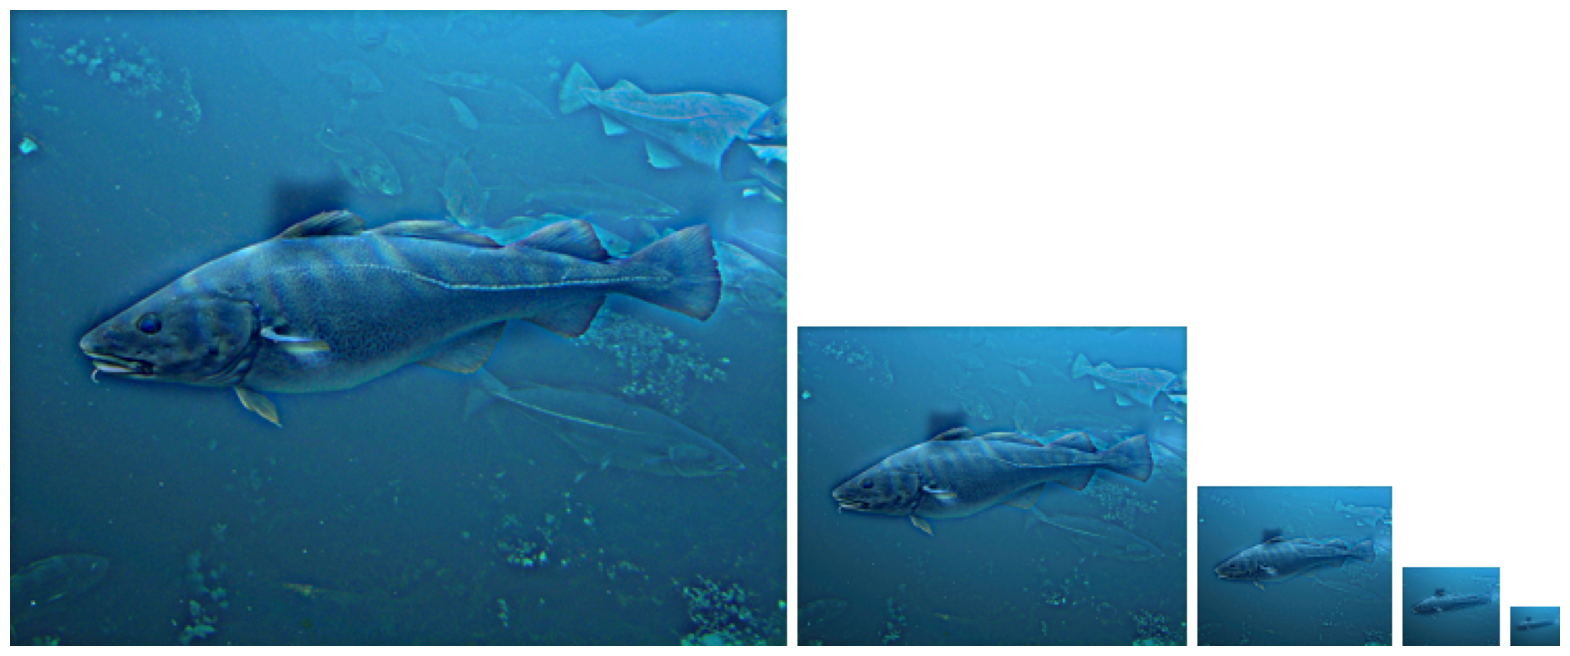
\includegraphics[height=15em]{./images/submarine_fish_hybrid.png}
        \caption{Submarine Fish Hybrid Image}
        \label{submarine_fish_hybrid}
\end{figure}

\chapter{Task Split}
\textbf{Raihan Uddin} was in charge of most of the implementation (coding) part. \\
\textbf{Sayan Das} was in charge of making this report in \LaTeX. He also contributed in identifying and fixing a bug in \textt{my\_imfilter} function where it was not working as intended when applying a rectangular filter. \\
\textbf{We Both} worked on reading the paper \cite{oliva2006} and helped each other understand it.

\chapter{Conclusion}
This project successfully implemented hybrid images using principles from Oliva et al.’s \cite{oliva2006} work. The results demonstrate the interplay of spatial frequencies in human perception, validating the paper’s claims. Future work could explore separable filters for speed.


\chapter*{Acknowledgement}
\addcontentsline{toc}{chapter}{Acknowledgement}

We would like to express our sincere gratitude to our supervisor, \textbf{Br. Bhaswarachaitanya} (Tamal Maharaj), Assistant Professor in the Department of Computer Science at \textit{Ramakrishna Mission Vivekananda Educational and Research Institute (RKMVERI)}, for his invaluable guidance, encouragement, and support throughout the course of this project. His expertise in computer vision and his insightful suggestions were instrumental in shaping this project.

We would also like to thank \textit{Ramakrishna Mission Vivekananda Educational and Research Institute} for providing the necessary resources and facilities that enabled the successful completion of this project.

Lastly, we extend our heartfelt thanks to our batch mates for their constant encouragement and understanding during the challenging phases of this project.

\renewcommand{\bibname}{References}
\begin{thebibliography}{9}
	\bibitem{oliva2006}
  Oliva, A., Torralba, A., \& Schyns, P. G. "Hybrid Images." \textit{ACM Transactions on Graphics (TOG)}, 2006.

  \bibitem{szeliski2010}
  Szeliski, R. "Computer Vision: Algorithms and Applications." \textit{Springer}, 2010.

\end{thebibliography}
\addcontentsline{toc}{chapter}{References}

\end{document}